\documentclass[twoside,twocolumn,10pt]{extarticle}

\usepackage{multirow}
\usepackage{textcase}
\usepackage{amsthm}
\usepackage{amssymb}
%\newtheorem{thm}{Theorem}
\theoremstyle{definition}
%\newtheorem{defn}[thm]{Definition} % definition numbers are dependent on theorem numbers
%\newtheorem{exmp}[thm]{Example}

\usepackage{blindtext} % Package to generate dummy text throughout this template 

\usepackage[sc]{mathpazo} % Use the Palatino font
\usepackage[T1]{fontenc} % Use 8-bit encoding that has 256 glyphs
\linespread{1.05} % Line spacing - Palatino needs more space between lines
\usepackage{microtype} % Slightly tweak font spacing for aesthetics

\usepackage[italian]{babel} % Language hyphenation and typographical rules
\usepackage[utf8]{inputenc}

\usepackage[hmarginratio=1:1,top=32mm,columnsep=20pt]{geometry} % Document margins
\usepackage[hang,small,labelfont=bf,up,textfont=it,up]{caption} % Custom captions under/above floats in tables or figures
\usepackage{booktabs} % Horizontal rules in tables
\usepackage{subcaption}

\usepackage{graphicx}
\usepackage{float}
\usepackage{listings}
\usepackage{color}

\definecolor{codegreen}{rgb}{0,0.6,0}
\definecolor{codegray}{rgb}{0.5,0.5,0.5}
\definecolor{codepurple}{rgb}{0.58,0,0.82}
\definecolor{backcolour}{rgb}{0.95,0.95,0.92}

\lstdefinestyle{mystyle}{
	backgroundcolor=\color{backcolour},   
	commentstyle=\color{codegreen},
	keywordstyle=\color{magenta},
	numberstyle=\tiny\color{codegray},
	stringstyle=\color{codepurple},
	basicstyle=\footnotesize,
	breakatwhitespace=false,         
	breaklines=true,                 
	captionpos=b,                    
	keepspaces=true,                 
	numbers=left,                    
	numbersep=5pt,                  
	showspaces=false,                
	showstringspaces=false,
	showtabs=false,                  
	tabsize=2
}
\lstset{style=mystyle}

\usepackage{lettrine} % The lettrine is the first enlarged letter at the beginning of the text

\usepackage{enumitem} % Customized lists
\setlist[itemize]{noitemsep} % Make itemize lists more compact

\usepackage{abstract} % Allows abstract customization
\renewcommand{\abstractnamefont}{\normalfont\bfseries} % Set the "Abstract" text to bold
\renewcommand{\abstracttextfont}{\normalfont\small\itshape} % Set the abstract itself to small italic text

\usepackage{titlesec} % Allows customization of titles
\renewcommand\thesection{\Roman{section}} % Roman numerals for the sections
\renewcommand\thesubsection{\roman{subsection}} % roman numerals for subsections
\titleformat{\section}[block]{\large\scshape\centering}{\thesection.}{1em}{} % Change the look of the section titles
\titleformat{\subsection}[block]{\large}{\thesubsection.}{1em}{} % Change the look of the section titles

\usepackage{fancyhdr} % Headers and footers
\pagestyle{fancy} % All pages have headers and footers
\fancyhead{} % Blank out the default header
\fancyfoot{} % Blank out the default footer
\fancyhead[C]{Riconoscimento Automatico della Prominenza in Italiano $\bullet$ Aprile 2017 $\bullet$ \textit{NLP}} % Custom header text
\fancyfoot[RO,LE]{\thepage} % Custom footer text

\usepackage{titling} % Customizing the title section

\usepackage{hyperref} % For hyperlinks in the PDF

% Title Section
\setlength{\droptitle}{-4\baselineskip} % Move the title up

\pretitle{\begin{center}\Huge\bfseries} % Article title formatting
\posttitle{\end{center}} % Article title closing formatting
\title{Riconoscimento automatico della Prominenza in Italiano:\\Reti Neurali Ricorsive} % Article title
\author{%
\textsc{Maxim Gaina} \\[1ex] % Your name
\normalsize Università di Bologna\thanks{Progetto per il corso di Elaborazione del Linguaggio Naturale, A.A. 2016/2017, prof. Fabio Tamburini.} \\ % Your institution
\normalsize \href{mailto:maxim.gaina@studio.unibo.it}{maxim.gaina@studio.unibo.it}
%\and % Uncomment if 2 authors are required, duplicate these 4 lines if more
%\textsc{Jane Smith}\thanks{Corresponding author} \\[1ex] % Second author's name
%\normalsize University of Utah \\ % Second author's institution
%\normalsize \href{mailto:jane@smith.com}{jane@smith.com} % Second author's email address
}
\date{\today} % Leave empty to omit a date
\renewcommand{\maketitlehookd}{%
\begin{abstract}
\noindent Nel parlato, la prominenza è un fenomeno percettivo che può influire pesantemente sulla semantica delle frasi pronunciate, per questo guadagna un ruolo fondamentale nella comunicazione umana. Sono stati svolti in passato diversi sperimenti per rilevare le sillabe prominenti all'interno di una frase, che prevedevano l'utilizzo di svariati strumenti offerti dall'ambito dell'Apprendimento Automatico e dai modelli Rule-Based. L'obiettivo di questo lavoro di progetto è impiegare, per la prima volta nella lingua italiana, le reti neurali ricorsive; valutare successivamente i benefici e infine confrontarli con i metodi precedentemente usati.
\end{abstract}
}

\begin{document}

\maketitle

\tableofcontents

\section*{Introduzione}
	\lettrine[nindent = 0.4em,lines=3]{O}\space\MakeTextLowercase{g}ni lingua possiede un suo insieme di tratti soprasegmentali, che caratterizzano la relativa sequenza lineare del parlato, e i vari rapporti tra foni che compongono tale sequenza. Tali informazioni prosodiche sono spesso cruciali per disambiguare espressioni sintattiche. Per capire, in breve, si prenda l'esempio riportato in \cite{bib:fenomeni-prosodici-prominenza}:
	\begin{itemize}
		\item[a.] \textit{È stato Luigi?}
		\item[b.] \textit{È stato Luigi.}
	\end{itemize}

	In italiano le frasi interrogative sono un esempio di come il profilo intonativo del parlante sia fondamentale, perché sintatticamente non sono marcate in alcun modo. Nel primo caso si ha un andamento finale ascendente, mentre nella frase dichiarativa tipicamente si tratta di un profilo finale discendente. In altri casi invece, il parlante accentua e/o allunga determinate parole, per concentrare l'attenzione dell'ascoltatore proprio in quel punto della sequenza.	 Si tratta ancora di informazioni difficilmente trasmissibili o per niente trasmissibili per vie sintattiche. I fenomeni prosidici sono quindi l'intonazione, il ritmo, la velocità di elocuzione, le pause e così via. L'oggetto di studio in questo lavoro è la \textbf{prominenza}, per la quale, più tardi, si cercherà di dare una definizione più esatta. Lo scopo ultimo, è quello di impiegare un particolare tipo di \textit{Reti Neurali Ricorsive} (\texttt{RNN}), cioè le \textit{Long-Short Term Memory} per l'identificazione automatica delle sillabe prominenti. Ancora meglio, si può dire che questo sia un problema di classificazione delle sillabe, prominenti e non, dove le caratteristiche di ogni sillaba dipendono dall'intero contesto in cui si trovano.
	
	Verrà qui esposto il modo in cui è stato affrontato il problema d'esame, preceduto però dalle informazioni necessarie allo studente per capire il problema trattato e il suo contesto, cioè dove si colloca all'interno del \textit{Natural Language Processing}. La relazione avrà quindi la seguente struttura:
	\begin{itemize}
		\item nella prima sezione si cercherà di definire meglio il dominio del problema, restringendolo;
		\item nella seconda sezione verranno spiegati brevemente i metodi di risoluzione del problema, in ambito \texttt{NLP};
		\item la terza sezione descriverà brevemente un particolare lavoro di sperimentazione già eseguito, e grazie al quale si ha a disposizione un corpus;
		\item la quarta sezione, sarà quella che approfondisce il nuovo strumento che si vuole usare per la costruzione del modello, cioè le \textit{Reti Neurali Ricorsive};
		\item verrà poi spiegato nello specifico il metodo di risoluzione e visualizzati i risultati ottenuti nella quinta sezione.
	\end{itemize}
	
\section{Il Fenomeno della Prominenza}\label{sec:prom}
	È stato detto che si vuole identificare automaticamente la prominenza, ma cosa significa esattamente? Non è proprio immediato dare una definizione, dal momento che gli studiosi addentratisi nel problema, arrivarono spesso a conclusioni divergenti, proponendo teorie e metodi diversi. Esaminando qualche rasségna in merito (\cite[Capitolo 1]{bib:fenomeni-prosodici-prominenza} e \cite{bib:prominence-by-acoustic-analyses}) è possibile vederlo. Talvolta i ricercatori vanno letteralmente in conflitto ridefinendo lo stesso termine, come per esempio lo \textit{stress}. Riprendendo però quanto detto in \cite{bib:prominence-by-acoustic-analyses}, si può così definire la prominenza:
	\theoremstyle{plain}
	\newtheorem{definition}{Definizione}
	\begin{definition}[Prominenza]\label{def:prosodic-prominency}
		La prominenza è un fenomeno percettivo, continuo nella sua natura, che enfatizza alcune unità linguistiche e segmentali rispettivamente al contesto che li circonda, e viene supportata da una complessa interazione fra parametri prosodici e fonetico-acustici.
	\end{definition}
	Da notare come la definizione fa riferimento a unità linguistiche segmentali all'interno dell'enunciato e, che queste siano dipendenti da altre unità linguistiche, che formano il contesto in cui si trovano. Questo sarà decisivo nel definire poi il metodo di risoluzione del problema. I parametri a cui si fa riferimento sono anche essi sempre stati oggetto di discussione. Uno degli obiettivi più importanti è sempre stato trovare un fenomeno linguistico/prosodico misurabile per supportare la percezione della prominenza. Fra tutti, e come suggerito in \cite{bib:prominence-by-acoustic-analyses}, si riporta come esempio uno studio che individua due impportanti attori al supporto della prominenza: il primo è il \textit{pitch accent} e riguarda il profilo della frequenza fondamentale; il secondo è il \textit{force accent}, più connesso a fenomeni acustici come intensità, durata del segmento e probabilmente altro. Il grado di prominenza dell'$i$-esimo segmento si può vedere come la somma di questi due parametri.

	Ci si potrebbe ora chiedere se la prominenza di un segmento si può stabilire con un \textit{sì/no}, su una scala ordinale oppure su una scala continua. La prominenza per sua natura è un fenomeno continuo, ma la sua discretizzazione può comunque essere attuata, dipende dall'approccio che si adotta per risolvere il problema.
	
	Un'altra domanda che sorge, è se lo studio della prominenza esige che vengano fatte delle distinzioni interlinguistiche. La risposta è sì, in quanto si può rilevare la presenza delle così dette \textit{tone languages}, in cui il profilo del pitch è correlato al significato stesso della parola pronunciata (il tailandese). Una versione più rilassata di questo principio è, per esempio, il giapponese, dove questo ancoraggio fra prominenza e semantica è molto più limitato, e le sillabe prominenti non portano con sé un allungamento o una profondità maggiore, ma semplicemente un profilo di pitch alto. Infine troviamo le \textit{stress languages}, nelle quali il tono non incide in alcun modo sui significati lessicali delle parole (inglese), ma le sillabe vengono \textit{stressate} in funzione comunicativa. Questo discorso è stato approfodito ulteriormente in alcuni studi, che classificano le lingue in funzione di due dimensioni: prominenza e pattern ritmico. La prima dimensione è importante da considerare, mentre la seconda interessa poco in questa sede.

\section{Riconoscimento Automatico della Prominenza}\label{sec:ric}
	Una volta definito e indagato il fenomeno della prominenza, è ora di chiedersi in che modo possa essere affrontato il problema del suo riconoscimento automatico. Si possono impiegare modelli computazionali che seguono due paradigmi diversi:
	\begin{enumerate}
		\item \textit{Rule Based}, consiste nel fornire regole formali per la risoluzione di un dato problema;
		\item \textit{Machine Learning}, viene retto un modello computazionale a partire da dati già esistenti, in questo caso da corpus annotati da esperti. 
	\end{enumerate}
	Riprendendo il comodo schema proposto in \cite{bib:prominence-by-acoustic-analyses}, si può dire che per quanto riguarda i sistemi rule-based, i principali vantaggi consistono nel permettere a chi si occupa di linguistica di controllare pienamente il comportamento degli algoritmi; di creare modelli che operano su diverse lingue; non richiedono grossi corpora annotati, e permettono di epsrimere il modello in termini linguistici. Solitamente però producono sistemi meno accurati. Si escludono tuttavia i sistemi rule-based in questo contesto, e ci si concentra sui metodi di apprendimento automatico. Questi ultimi permettono di avere sistemi altamente performanti; permettono una più veloce classificazione e apprendono a partire dai dati. L'ultimo aspetto elencato è anche un punto dolente in \texttt{NLP}, sono infatti necessari grossi corpora annotati che non sempre si hanno a disposizione. La creazione di corpora può richiedere enormi sforzi umani ed economici, in più gli annotatori umani non sono mai al $100\%$ concordi sulla parte prominente delle frasi. Si noti che in ambito \textit{Machine Learning} (\texttt{ML}) esistono metodi di apprendimento supervisionati e metodi apprendimento non supervisionati, e la necessità di avere queste risorse annotate è presente nei sistemi supervisionati. In \cite[Sezione 4.2]{bib:fenomeni-prosodici-prominenza} è stato proposto un metodo non supervisionato, che, data la segmentazione dell'enunciato, fa uso di una funzione di prominenza per fissarla su una scala continua. L'obiettivo di sistemi del genere è quello di liberare dalla necessità di avere larghi corpus annotati. In questo lavoro si cercherà di costruire tuttavia, un sistema supervisionato con diverse fasi di apprendimento. 
	
	Per quanto riguarda la segmentazione degli enunciati, il problema è simile. Se il corpus è creato da risorse umane si possono usare le segmentazioni eseguite a mano. Negli ambienti più realistici però, queste informazioni non si hanno a disposizione. Anche in merito sono stati fatti degli studi per identificare automaticamente delle pseudo sillabe e i relativi nuclei.
	
	\subsection{Metriche di valutazione}
		Si intende in questa relazione riportare i risultati di sperimentazioni già fatte e confrontarli con il lavoro qui svolto, per questo è necessario usare delle metriche ben precise. Tali metriche sono tipiche dell'ambito \texttt{ML}, e l'importanza di ognuna di loro varia a seconda del tipo di problema e quindi dei modelli usati. Verranno ora viste quelle fondamentali per affrontare il problema posto.
		
		Dato un insieme di sillabe, siano i seguenti totali calcolati:
		\begin{itemize}
			\item[$a$:] corrette previsioni di non prominenza;
			\item[$b$:] scorrette previsioni di prominenza;
			\item[$c$:] scorrette previsioni di non prominenza;
			\item[$d$:] corrette previsioni della prominenza.
		\end{itemize}
		In altre parole sarebbero, rispettivamente, le sillabe scartate correttamente; i falsi allarmi; le mancate individuazioni e le corrette individuazioni della prominenza. A partire da questi parametri si può già definire l'\textbf{accuratezza} $AC$, che esprime la percentuale di corrette classificazioni rispetto al totale numero delle sillabe:
		\begin{equation}\label{eq:ac}
			AC = (a + d) / (a + b + c + d)
		\end{equation}
		La metrica \textbf{recupero} $R$ invece, abbondantemente usata anche nell'ambito dell'\textit{Information Retrieval} (per esprimere la percentuale di documenti utili trovati sul totale di quelli rilevanti), rappresenta qui la percentuale di sillabe prominenti correttamente identificate, ovvero:
		\begin{equation}\label{eq:r}
			R = d / (c + d)
		\end{equation}
		La \textbf{precisione} $P$ è la percentuale di corrette classificazioni di sillabe prominenti:
		\begin{equation}\label{eq:p}
			P = d / (b + d)
		\end{equation}
		Quando gli elementi da classificare sono distribuiti in modo sbilanciato, la metrica $AC$ può non essere il miglior indicatore delle prestazioni del modello. Si vedrà infatti, anche se è intuibile, che le sillabe prominenti sono una minoranza. Siamo anche di fronte a una situazione in cui, per esempio, il richiamo $R$ come metrica non è strettamente più importante della precisione. Per valutare le prestazioni di un sistema, si ricorre quindi a una metrica combinata che tiene conto di entrambe, che può essere l'\textbf{F-Score} così definito:
		\begin{equation}\label{eq:f}
			F1 = 2 \cdot \frac{P \cdot R}{P + R}
		\end{equation}
		Viene chiamata $F1$ perché si tratta del caso specifico in cui nella formula generalizzata dell'\textit{F-score} $\beta$ viene impostato a $1$, così che precisione e richiamo abbiano lo stesso peso.
	
\section{Il Corpus Annotato}\label{sec:corpus}
	Per raggiungere l'obiettivo verrà usato lo stesso corpus dell'eperiménto \cite{bib:prominence-detection-italian}, che ora si andrà ad analizzare per avere un'adeguata comprensione.
	
	\subsection{L'esperimento orignario}
		Esiste un'altra famiglia di sistemi \texttt{ML}, le \textit{Probabilistic Graphical Models} (\texttt{PGM}). Esse sono in grado di elaborare sequenze di dati in input facendo previsioni su quelle in output, considerando sia la sequenza di input attuale che quella di output precedente. Data quindi una generica sequenza di vettori $\{v^x_1, ..., v^x_n\}$ in input, contenenti le features, e data la sequenza $\{y_1, ..., y_n\}$ in output, i modelli di tipo \texttt{PGM} etichettano ogni $y_i$ nel modo più probabilmente opprtuno. Le \texttt{PGM} però sono un insieme di convinzioni per strutturare i modelli, e più tipi di \texttt{PGM} sono state usate in \cite{bib:prominence-detection-italian} per il riconoscimento automatico della prominenza.
	
		Il corpus è stato costruito a partire da conversazioni di persone italiane provenienti dall'area di Pisa, sia femmine che maschi. Il corpus contiene un totale di $120$ espressioni segmentate, con una lunghezza media di $18$ sillabe che vanno da un minimo di $9$ a un massimo di $35$. Ai partecipanti fu chiesto poi di individuare quali fosse secondo loro le prominenze negli enunciati, presentando loro le segmentazioni. L'intero procedimento, in realtà più complesso, è descritto nel documento originale. Le sillabe sono state poi raggruppate in base alla percentuale di convergenza di etichettature da parte di tutti. Questi significa che, dato che ogni sillaba è stata valutata da $10$ persone, essa può essere giudicata prominente da più di $6$, $7$, $8$ o $9$ persone. Infine, sono state selezionate le sillabe convergenti nell'$80\%$ dei casi come prominenti, che sono il $23,56\%$ del totale. È stato fatto poi un'altro tipo di selezione, in cui il peso più importante veniva considerato il livello di affidabilità dei giudici. In questo caso risultavano prominenti il $33,46\%$ delle sillabe nel corpus.
		
	\subsection{Le features}
		\begin{table*}[h]
			\centering
			\caption{Gerarchia dei fenomeni coinvolti nel riconoscimento automatico della Prominenza}
			\begin{tabular}{l|c|c|c|c}
				\hline
				Fenomeni percettivi & \multicolumn{4}{c}{Prominenza}                                                                                                                                                               \\ \hline
				Fenomeni prosodici  & \multicolumn{2}{c}{Stress}                                         & \multicolumn{2}{c}{Pitch accent}                                                                                       \\ \hline
				Fenomeni acustici   & durata & \begin{tabular}[c]{@{}c@{}}enfasi\\ spettrale\end{tabular} & \begin{tabular}[c]{@{}c@{}}movimenti\\ in F0\end{tabular} & \begin{tabular}[c]{@{}c@{}}intensità\\ globale\end{tabular} \\ \hline
			\end{tabular}
			\label{tab:gerarchia}
		\end{table*}
		\begin{table*}[h]
			\centering
			\caption{Il migliore sistema \texttt{PGM} (\textit{Latent-Dynamic Conditional Neural Fields}) al variare del metodo di selezione delle sillabe prominenti.}
			\label{tab:pgm}
			\begin{tabular}{lrrrr}
				\hline
				& \multicolumn{1}{c}{Accuratezza AC} & \multicolumn{1}{c}{Precisione P} & \multicolumn{1}{c}{Richiamo R} & \multicolumn{1}{c}{F-score F1} \\ \hline
				Convergenza 80\% & \textbf{0.875} & 0.788 & 0.658 & 0.716 \\
				Best-3 & 0.855 & \textbf{0.831} & \textbf{0.718} & \textbf{0.770} \\ \hline
			\end{tabular}
		\end{table*}
		Ogni sillaba all'interno dell'espressione ha un determinato numero di caratteristiche. Come è stato già accennato, ci saranno principalmente due attori a determinare le features: pitch-accent e force-accent. Senza andare troppo nel dettaglio, le caratteristiche di ogni sillabe sono le seguenti:
		\begin{enumerate}
			\item \textbf{durata nucelo}, normalizzata rispetto alla media e alla varianza del nucleo all'interno dell'espressione;
			\item \textbf{spectral emphasis}, feature anch'essa normalizzta con \texttt{z-score};
			\item \textbf{movimenti del pitch}, feature calcolata a partire da parametri forniti dal modello \texttt{TILT} e con l'ausilio di specifici algoritmi per individuare il picco;
			\item \textbf{intensità complessiva};
			\item \textbf{durata sillaba}, valore ricavato come per la durata del nucleo, ma riguardante l'intera sillaba.
		\end{enumerate}
		
		A parte la durata della sillaba, tutte le features sono calcolate nel dominio del nucleo della sillaba. La comprensione di come queste caratteristiche si inseriscano nel quadro dello studio (durata della sillaba a parte), viene facilitata dalla gerarchia dei fenomeni proposta nel \cite[Capitolo 3]{bib:fenomeni-prosodici-prominenza}, e riproposta nella Tabella \ref{tab:gerarchia}. Il fenomeno percettivo della prominenza è basato sui fenomeni prosodici dello \textit{stress}	e il \textit{pitch accent}, a loro volta correlati a fenomeni acustici ricavabili da parametri fisici dell'enunciato. Inoltre, ogni fenomeno prosodico è sufficiente per individuare il fenomeno della prominenza, singolarmente o in presenza dell'altro.
		
	\subsection{Risultati}
		
		Per le \texttt{PGM} è stato usato un training set di $100$ espressioni mentre il test set ne conteneva $20$. La Tabella \ref{tab:pgm} riporta le prestazioni raggiunte, senza (ricordiamo) l'utilizzo di alcuna caratteristica linguistica, solo tramite informazioni acustiche. I risultati ottenuti non possono essere comparati con altri studi nel settore, dato che sarebbe necessario avere lo stesso corpus.
		
		In \cite{bib:prominence-detection-italian} è stato anche fatto vedere quanto le \texttt{PGM}, e in particolare le \texttt{LDCNF}, siano meglio in confronto alle \textit{Support Vector Machines} (\texttt{SVM}). L'\textit{F-measure} infatti migliora di mezzo punto, da $0.665$ a $0.716$ per il criterio della convergenza, e di $0.38$ punti per il criterio \textit{best-3}. Si cercherà di fare un confronto simile usando le reti neurali ricorsive, andando a vedere che miglioramento sono in grado di apportare alla causa.
	
\section{Reti Neurali Ricorsive}\label{sec:rnn}
	\begin{figure*}[h]
		\centering
		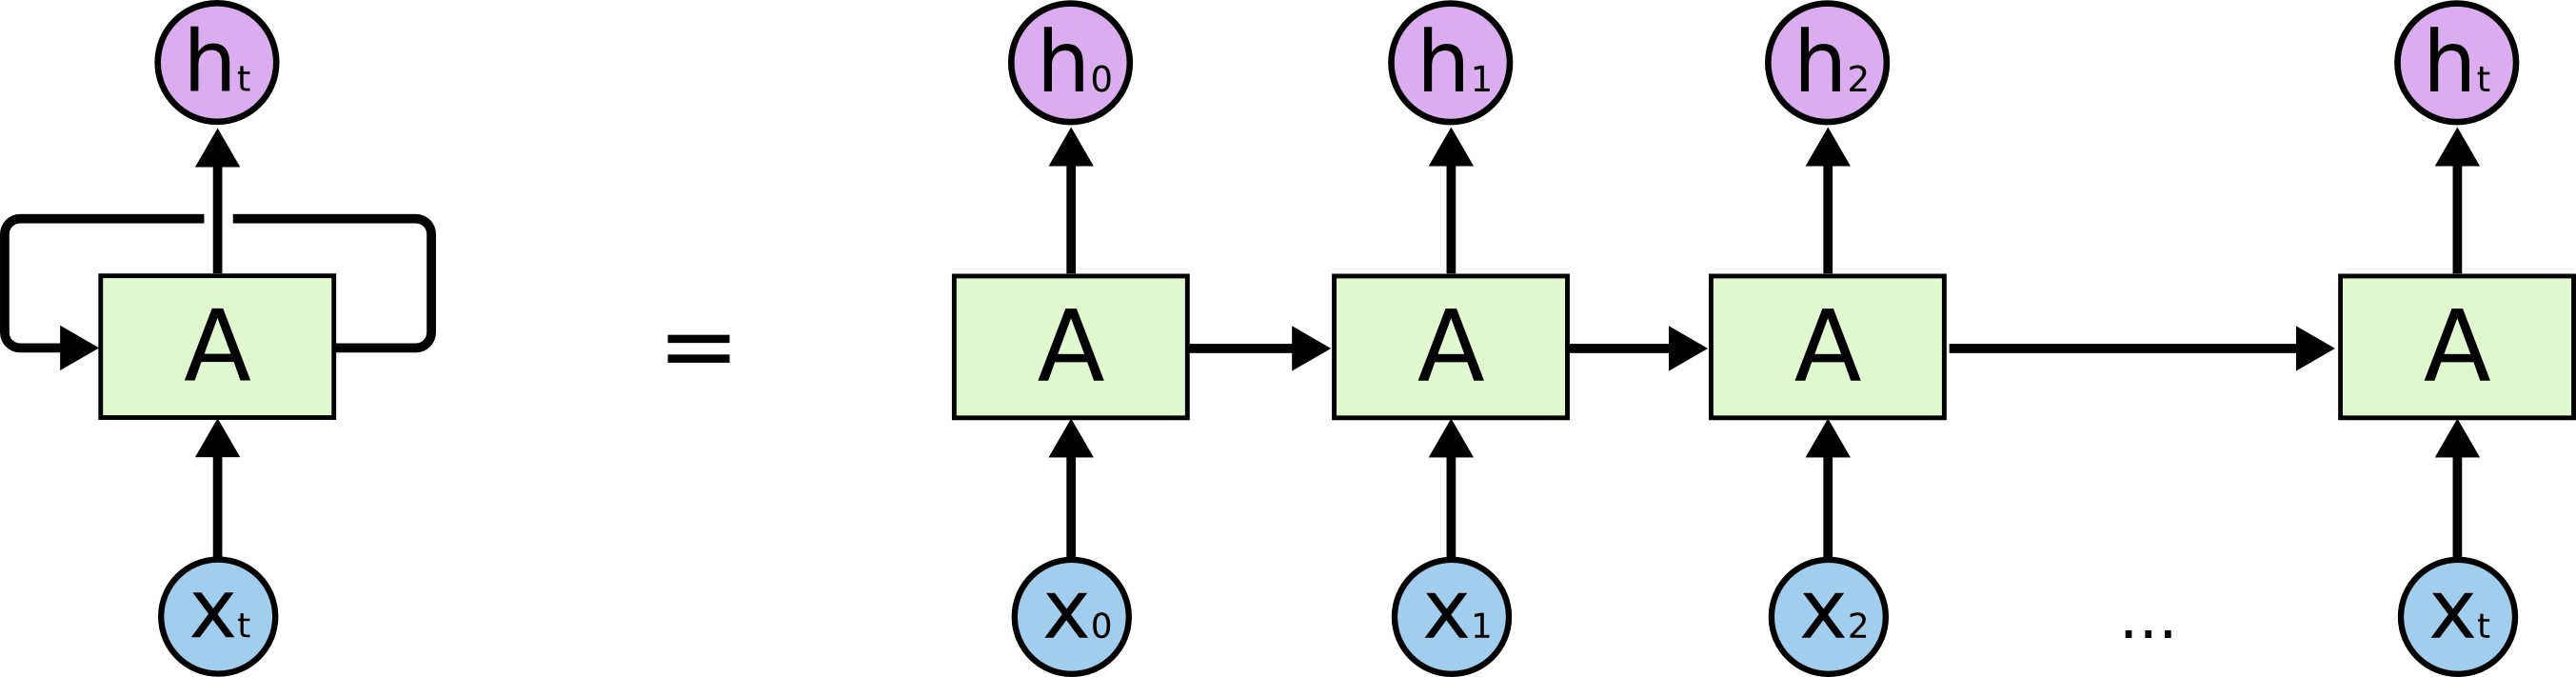
\includegraphics[scale=.4]{img/rnn.png}
		\caption{\textit{Unrolling} di una rete neurale ricorsiva}
		\label{fig:unroll}
	\end{figure*}
	La Definizione \ref{def:prosodic-prominency} della prominenza classifica tale fenomeno come continuo e marcato rispettivamente al contensto che lo circonda. Questo significa che le tradizionali reti neurali non possono affrontare un problema del genere, non è chiaro infatti come possano analizzare per esempio, il significato di una parola quando esso dipende da quanto è stato precedentemente detto.
	
	Le \textit{Reti Neurali Ricorsive} (\texttt{RNN}) sembrano ovviare a questo problema. Le \texttt{RNN} sono un tipo di rete contenente al loro interno dei cicli, ciò rende possibile che le stesse informazioni persistano al loro interno.

	Nella Figura \ref{fig:unroll} si può vedere come, preso un ciclo, una \texttt{RNN} si può interpretare come una successione di copie della stessa rete. La loro struttura \textit{a catena} si adatta perfettamente all'elaborazione di sequenze e liste. L'interpretazione è la seguente: data un porzione di rete $A$, essa guarda l'input $x_t$ e produce l'output $h_t$, permettendo tramite il loop di passare l'informazione dal passo $t$ a $t + 1$. Una \texttt{RNN} può quindi guardare dietro nel tempo, individuare una dipendenza fra passato e presente e quindi produrre l'output più opportuno. La domanda ora è la seguente: \textit{quanto} indietro nel tempo? Sfortunatamente, le \texttt{RNN} perdono efficacia man mano che la distanza tra passato interessante e presente aumenta.
	
	\subsection{Long Short Term Memory}\label{subsec:lstm}
		Le \textit{Long Short Term Memory} (\texttt{LSTM}) sono un particolare tipo di \texttt{RNN} capaci di apprendere dipendenze a lungo termine. Infatti, le \texttt{LSTM} sono state proposte proprio per ovviare al problema delle \texttt{RNN} precedentemente descritto. I moduli, in questo tipo di architettura (Figura \ref{fig:lstm}), racchiudono al loro interno più layer con funzione di attivazione \texttt{sigmoid} e \texttt{tanh} che interagiscono fra loro in maniera ben specifica.
		
		\begin{figure*}[h]
			\centering
			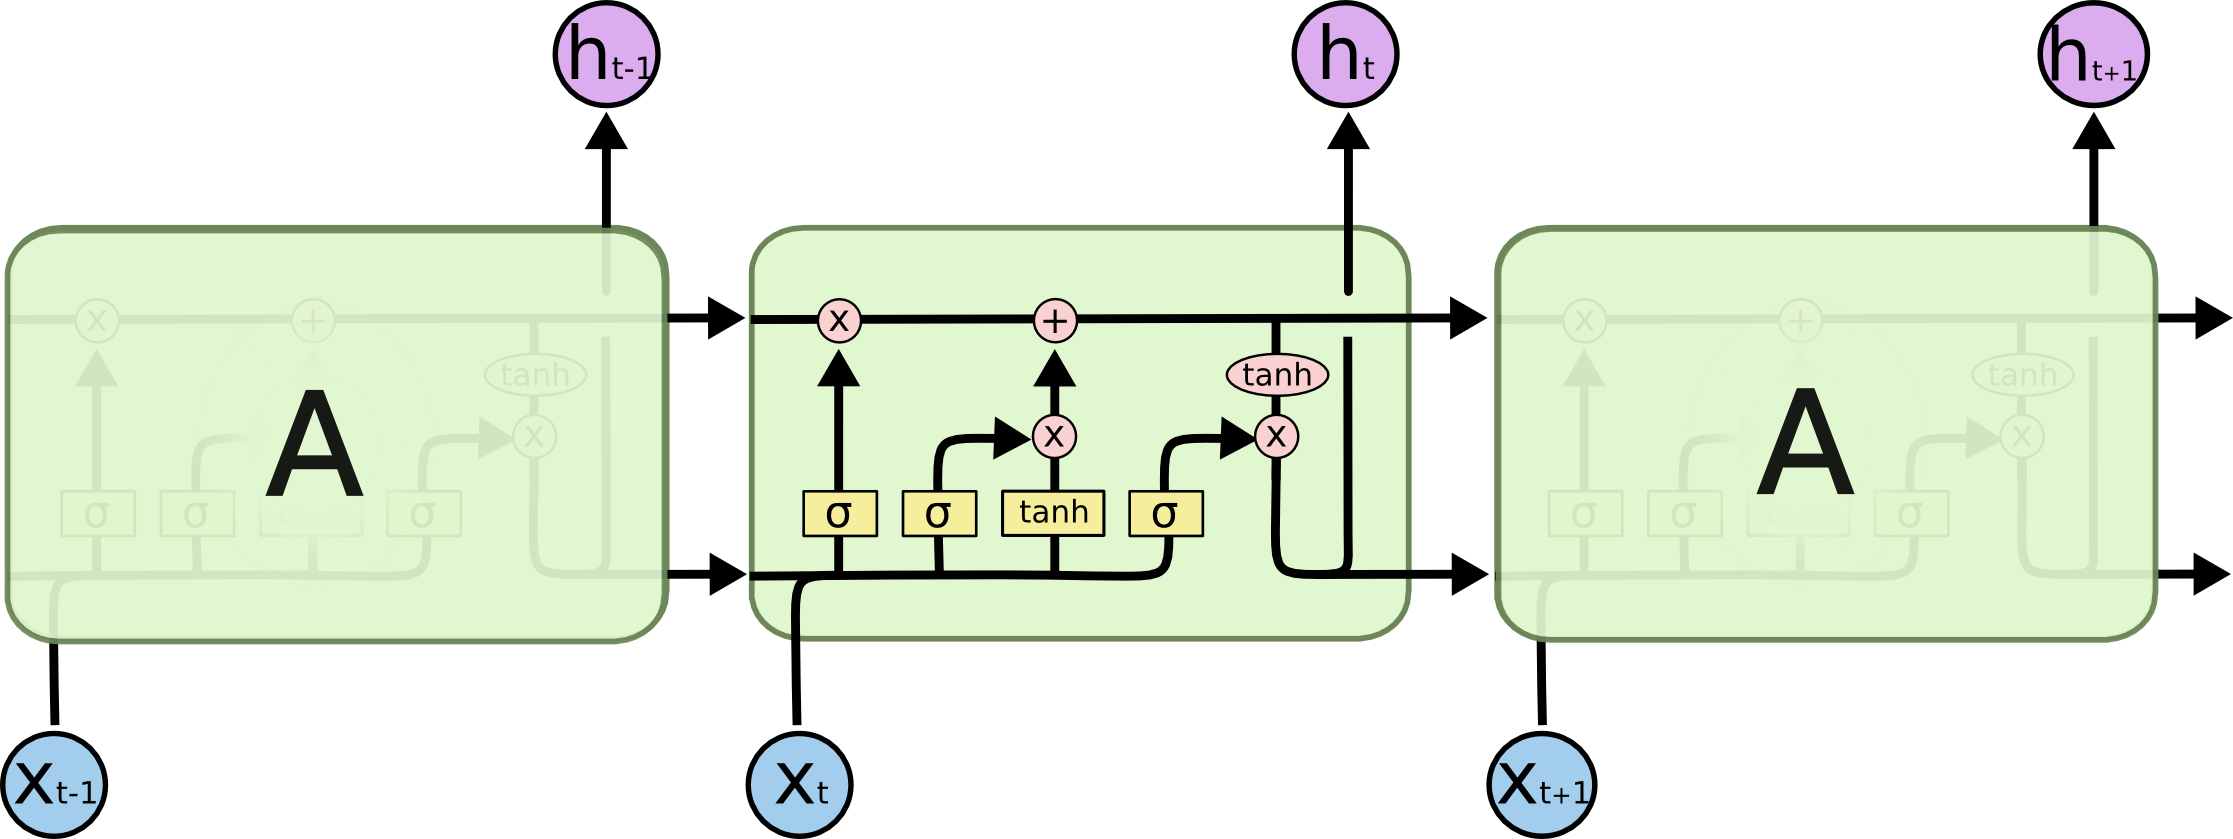
\includegraphics[scale=.5]{img/lstm.png}
			\caption{Esempio di struttura interna alla base delle \textit{Long Short Term Memory (\texttt{LSTM})}}
			\label{fig:lstm}
		\end{figure*}
	
		L'idea alla base è che la \texttt{LSTM} può rimuovere o aggiungere informazioni allo stato della sua cella. Tali scelte vengono influenzate da strutture chiamate \textit{porta} (o \textit{gate}). Una porta fa passare l'informazione nello stato della cella in maniera ottimale, dato che la porta stessa non è altro che uno strato di rete neurale con funzione di attivazione sigmoidea (cella $\sigma$ in Figura \ref{fig:lstm}). Si ricordi che il range di $\sigma$ è compreso fra $0$ (\textit{non far entrare nulla}) e $1$ (\textit{fai entrare tutto}), è necessario ricordare anche che gli strati di tipo \texttt{tanh} restituiscono valori compresi fra $1$ e $-1$. Seguono brevemente i passi che ci sono dietro al funzionamento di una \texttt{LSTM}, spiegando i principi sottostanti senza addentrarsi troppo nella loro complessità.
	
		\begin{figure*}[h]
			\centering
			\begin{subfigure}[b]{.496\textwidth}
				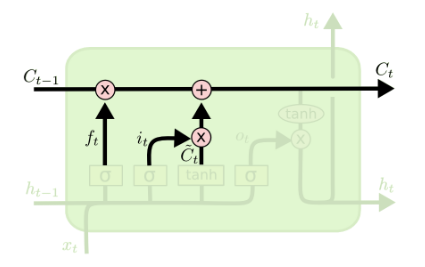
\includegraphics[width=\textwidth]{img/inside-lstm.png}
				\caption{Parametri calcolati nelle prime fasi}
			\end{subfigure}
			\begin{subfigure}[b]{.496\textwidth}
				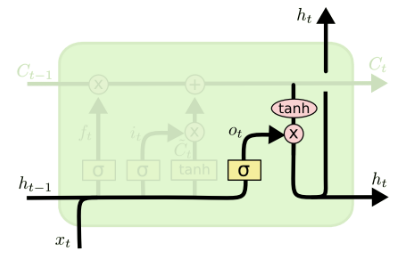
\includegraphics[width=\textwidth]{img/inside-lstm2.png}
				\caption{Parametri calcolati nelle ultime fasi}
			\end{subfigure}
			\caption{Mappa dei parametri interni a una \texttt{LSTM}}
			\label{fig:parmap}
		\end{figure*}
		
		\paragraph{Informazioni da dimenticare}
			All'arrivo dell'input $x_t$, la prima cosa da fare è decidere quale informazione precedentemente ottenuta va buttata via. Viene prelevato l'output $h_{t - 1}$ e l'input attuale $x_t$ (Figura \ref{fig:lstm}), e restituito il valore compreso fra $0$ e $1$ per ogni numero nello stato della cella $C_{t - 1}$. L'equazione \ref{eq:ft} esprime il calcolo dei relativi pesi e bias dello strato $\sigma$, con il dovuto output.
			\begin{equation}\label{eq:ft}
				f_t = \sigma(W_f \cdot [h_{t - 1}, x_t] + b_f)
			\end{equation}
			$f_t$ è da associare alla parola inglese \textit{forget}, letteralmente \textit{dimentica al passo t}.
		
		\paragraph{Decidere quali informazione assorbire}
			Il prossimo passo è quello di decidere quali informazioni assorbire nello stato della cella. In questa fase è coinvolto un'altro strato $\sigma$, detto \textit{porta di input}, e uno strato \texttt{tanh} che crea un vettore di valori candidati con i queli \textit{potrebbe} essere aggiornato il nuovo stato. L'output dello strato $\sigma$ è dato dall'equazione \ref{eq:it}, mentre il calcolo dell'ipotetico stato aggiornato $\tilde{C_t}$ viene espresso dall'equazione \ref{eq:futurec}.
			\begin{equation}\label{eq:it}
				i_t = \sigma(W_i \cdot [h_{t - 1}, h_t] + b_i)
			\end{equation}
			\begin{equation}\label{eq:futurec}
				\tilde{C_t} = tanh(W_C \cdot [h_{t - 1}, h_t] + b_C)
			\end{equation}
			
		\paragraph{Aggiornamento dello stato}
			Una volta deciso cosa si vuole ricavare dal nuovo input, è il momento di aggiornare effettivamente $C_{t - 1}$ per ottenere $C_t$.
			\begin{enumerate}
				\item per dimenticare quello che è stato deciso viene eseguito $C_{t - 1} \cdot f_t$;
				\item per assorbire quello che è stato ritenuto necessario viene eseguito $\tilde{C_t} \cdot i_t$;
				\item i risultati dei due passi sopra vengono sommati (Equazione \ref{eq:newstate}).
			\end{enumerate}
			\begin{equation}\label{eq:newstate}
				C_t = f_t * C_{t - 1} + i_t * \tilde{C_t}
			\end{equation}
		
		\paragraph{Output}
			Una volta creato lo stato $C_t$ bisogna decidere l'output, esso sarà basato sempre sullo stato della cella, ma conterrà solo alcuni suoi valori filtrati. Ancora una volta, uno strato $\sigma$ decide quali saranno le parti di $\tilde{C_t}$ a formare $o_t$. $o_t$ verrà poi moltiplicato per lo stato $C_t$, filtrato da un \textit{layer} \texttt{tanh}, ottenendo così l'output finale $h_t$, che verrà usato al passo $t$ per ricavare $h_{t + 1}$.
			\begin{equation}
				o_t = \sigma(W_o \cdot [h_{t - 1}, x_t] + b_o)
			\end{equation}
			\begin{equation}
				h_t = o_t * tanh(C_t)
			\end{equation}
			La \textit{mappa} dei parametri appena esposti si possono intuitivamente osservare nella Figura \ref{fig:parmap}.
		
		La breve spiegazione qui fornita riflette i concetti base\footnote{Cristopher Olah, \emph{\href{http://colah.github.io/posts/2015-08-Understanding-LSTMs/}{Understanding LSTM Networks.}}}, esistono comunque parecchie versioni concettuali che variano sensibilmente e ancora più numerose sono le implementazioni.
		
	\subsection{Un problema di Sequenze}
		Il motivo per cui le \texttt{LSTM} sono adatte a trattare il riconoscimento automatico della prominenza è che sono in grado di elaborare \textit{sequenze} di vettori\footnote{Andrej Karpathy, \emph{\href{http://karpathy.github.io/2015/05/21/rnn-effectiveness/}{The Unreasonable Effectiveness of Recurrent Neural Networks.}}}, che rappresentano le \textit{features}, e restituire sequenze di dimensione fissa a piacere. Ed è anche il motivo per il quale vengono usate nel trattamento dei video, testi, immagini, problemi \texttt{NLP}, e altro. I problemi sono risolvibili (classificazione, previsione, ecc...) tramite forme di mappatura rappresentati nella Figura \ref{fig:seqs}.	In base al tipo di mapping scelto, varia l'architettura della \textit{Rete Neurale Ricorsiva}. Vedremo nella prossima sezione come risulta l'architettura nel nostro caso.
		
		\begin{figure*}[h]
			\centering
			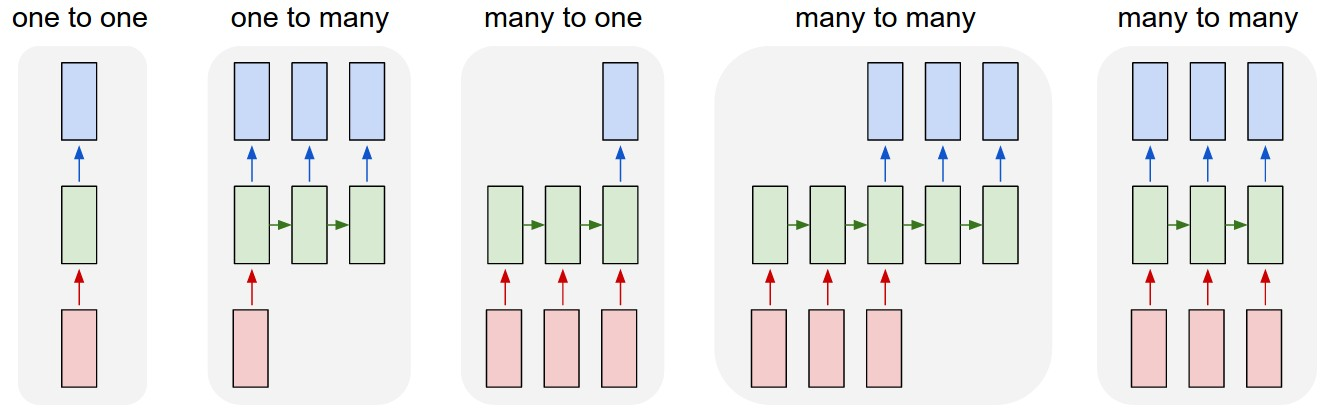
\includegraphics[scale=.3]{img/seqs.jpeg}
			\caption{Problemi \textit{sequence-to-sequence} trattabili con le \texttt{RNN}}
			\label{fig:seqs}
		\end{figure*}

\section{Costruzione del Modello}\label{sec:building}
	Le \texttt{LSTM} precedentemente riportare, così come le reti neurali in genere, hanno diverse varianti e implementazioni. Per la realizzazione del modello è stato scelto \texttt{Keras} \cite{bib:chollet2015keras}, che è un \texttt{API} ad alto livello per diverse tipologie di reti neurali. Il principio che sta alla base di \texttt{Keras} è che la chiave per fare della buona ricerca consiste nel rendere minima la distanza fra l'idea e la sua realizzazione, si ha quindi una libreria parecchio potente a disposizione. È scritta in \texttt{Python}, e si può scegliere l'implemtazione basata su \texttt{Theano} o \texttt{TensorFlow}.
	
	In \texttt{Keras}, un modello è una pila di diversi strati (reti neurali) collegati fra loro, dove gli input entrano nello strato d'ingresso e fuoriescono risultati dallo strato di uscita. Si possono però unire diversi modelli in uno unico, combinando i loro output tramite gli strati di classe \texttt{Merge}.
	
	Per la realizzazione di questo progetto è stato usato \texttt{Python 3.5} e \texttt{Keras 1.2.2}. Verranno ora descritti brevemente gli strati impiegati nel tentativo di costruire la miglior rete neurale.
	
	\paragraph{Masking Layer}
		Lo strato in questione ha il compito di \textit{mascherare} i valori in input che sono uguali a un certo valore. Va tenuto presente che la rete neurale prenderà in input sempre frasi di lunghezza $n = 34$, me le espressioni più corte avranno (alla fine) vettori di zeri al posto delle features mancanti. In questo caso il valore da mascherare sarà quindi $\{0, 0, 0, 0, 0\}$:
		\begin{center}
			\begin{verbatim}
				model.add(Masking(
					mask_value = [0.0, 0.0, 0.0, 0.0, 0.0]))
			\end{verbatim}
		\end{center}
		Significa letteralmente che la rete neurale non cercherà di imparare a partire dai valori mascherati.
	
	\paragraph{Dense Layer}
		È lo strato che implementa una tipica rete neurale densamente connessa, con un arbitrario numero di nodi, funzione di attivazione e altro.
		
	\paragraph{LSTM Layer}
		È l'implementazione di una rete \texttt{LSTM} descritta in \ref{subsec:lstm}.
		
	\paragraph{Dropout Layer}
		L'obiettivo principale dello strato di \texttt{Dropout} è quello di prevenire l'overfitting, e viene spesso abbinato ai layer \texttt{LSTM}. Si tratta di una tecnica in cui nella fase di training un numero casuale di unità della rete vengono ignorate, costringendo i \textit{neuroni} (o celle) attive a imparare anche per conto di quelli mancanti. L'effetto (desiderato) è che l'intera rete diventa meno sensibile agli specifici pesi di ogni unità di rete. Ogni volta, i nodi selezionati vengono gettati fuori dal quadro con una certa probabilità (per esempio il 50\%).
		\begin{center}
			\begin{verbatim}
				model.add(Dropout(0.5))
			\end{verbatim}
		\end{center}
	
	\paragraph{TimeDistributed Wrapper}
		Non si tratta di uno strato bensì di uno \texttt{wrapper}. Prende in input un determinato layer che viene applicato ad ogni intervallo di tempo dell'input della rete. Questo wrapper farà quindi sì che la rete restitiuisca sequenze.
		\begin{center}
			\begin{verbatim}
				model.add(TimeDistributed(Dense(5)))
			\end{verbatim}
		\end{center}
	
	\subsection{Costruzione della rete}
		Avendo estratto le features di sillabe per ogni enunciato all'interno del corpus e le relative classificazioni di prominenza, viene individuata la frase contenente più sillabe in assoluto. Ogni sillaba possiede un vettore di $5$ features e la sua classificazione binaria \textit{prominente / non prominente}, e la frase più lunga contiene $n = 34$ sillabe. Si ha quindi il problema di mappare correttamente i seguenti insiemi:
		\begin{equation}
			\{v_1, ..., v_n\} \rightarrow \{p_1, ..., p_n\}
		\end{equation}
		Nella Figura \ref{fig:seqs} ciò corrisponde al modello \textit{many to many}, il quinto tipo. Sappiamo cosa è $v_i$, è necessario ora decidere cosa è $p_i$. All'inizio l'assunzione era che $p_i \in \{0, 1\}$ per indicare la non prominenza e il contrario, ma tutti i modelli costruiti intorno a questa scelta erano davvero scadenti ($F1$ non più del $46\%$). Tali modelli prevedevano, oltre i dovuti layer \texttt{LSTM}, l'utilizzo di \texttt{Masking} come layer di input e uno strato \texttt{Dense(34)} che ritornasse $0$ e $1$ per ogni sillaba in ingresso.
		
		Per cercare altre vie è stato asserito che $p_i \in \{\{0, 1\}, \{1, 0\}\}$, dove $1$ nella prima posizione stava per indicare che la sillaba non è prominente e nella seconda posizione il contrario. Per realizzare la cosa è stato impostato \texttt{TimeDistributed(Dense(2))} come strato finale, con funzione di attivazione \texttt{softmax}, in modo che ritornasse dati in dimensione $(34, 2)$, con probabilità accumulata in una delle due posizioni. I sistemi risultanti davano un migliorato score $F1$ ma l'accuratezza era parecchio calata, a circa il $60\%$.
		
		È stato infine intuito che la \textit{sporcizia} è data dalle sillabe mancanti: per qualche motivo lo strato \texttt{Masking} non dava i risultati sperati, e le sillabe mancanti venivano denotate dalla rete come un'assoluta incertezza in cui alle entrambi posizioni veniva assegnata una probabilità del $50\%$.  Il problema è stato raggirato togliendo tale strato e, decidendo di non ignorare le sillabe mancanti, ma di classificare pure quelle. L'output per ogni \textit{timestep} è quindi diventato $p_i \in \{\{1, 0, 0\}, \{0, 1, 0\}, \{0, 0, 1\}\}$ (per indicare rispettivamente non prominenza, prominenza e assenza). Infinie, l'ultimo layer \texttt{Dense(3)} con attivazione \texttt{softmax} e dentro uno wrapper \texttt{TimeDistributed}, avrebbe concentrato le probabilità in una delle $3$ posizioni.
		
	\subsection{Bidirectional \texttt{LSTM}}
		\begin{figure}
			\centering
			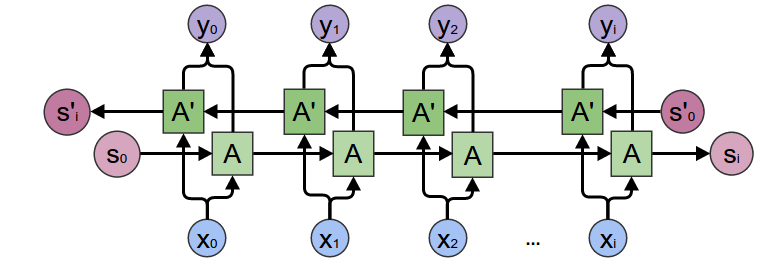
\includegraphics[scale=.26]{img/blstm.png}
			\caption{Architettura astratta di una rete \texttt{BLSTM}}
			\label{fig:blstm}
		\end{figure}
		\begin{figure*}[ht!]
			\centering
			\caption{Costruzione del modello con \texttt{Keras}}
			\lstinputlisting[language=Python]{code/seq.py}
			\label{fig:modelcode}
		\end{figure*}
		\begin{table*}[]
			\centering
			\caption{Risultati ottenuti in seguito al lavoro di progetto, confrontati con il modello \texttt{LDCNF}.}
			\label{tab:results}
			\begin{tabular}{lcccc}
				\hline
				Modello              & \multicolumn{1}{l}{Accuratezza A} & \multicolumn{1}{l}{Precisione P} & \multicolumn{1}{l}{Richiamo R} & \multicolumn{1}{l}{Fmeasure F1} \\ \hline
				LDCNF best-3         & 85.50\%                           & 83.10\%                          & 71.80\%                        & 77.00\%                         \\
				LSTM\_17             & 91.99\%                           & 88.66\%                          & 87.13\%                        & 87.88\%                         \\
				LSTM\_34             & 92.27\%                           & 88.84\%                          & 87.84\%                        & 88.33\%                         \\
				\textbf{BLSTM\_17x2} & \textbf{94.28\%}                  & \textbf{91.57\%}                 & \textbf{91.25\%}               & \textbf{91.41\%}                \\ \hline
			\end{tabular}
		\end{table*}
		In base a prove empiriche la scelta finale è ricaduta sulla seguente architettura, in ordine:
		\begin{itemize}
			\item \texttt{LSTM} Layer;
			\item \texttt{Dropout} Layer;
			\item \texttt{Dense} layer contenuto dentro wrapper \texttt{TimeDistributed}.
		\end{itemize}
		In seguito ad alcune ricerche è stato scoperto che una versione di rete \texttt{LSTM}, ovvero le \textit{Bidirectional} \texttt{LSTM} (\texttt{BLSTM}), si comportano molto bene nei problemi di \textit{sequence-labeling} in ambito \texttt{NLP} (come nel seguente lavoro \cite[Capitolo 5]{bib:blstm}). Sono state messe alla prova, incapuslando una rete \texttt{LSTM} dentro uno wrapper \texttt{Bidirectional} comodamente offerto da \texttt{Keras}. L'idea che sta alla base delle reti \texttt{BLSTM} è che un dato output $y_t$ non dipende solo dalle esperienze passate ma anche da quelle $future$. Esse racchiudono infatti uno strato \texttt{LSTM} \textit{forward} un'altro detto \texttt{backward} (Figura \ref{fig:blstm}), creando una doppia dipendenza. Probabilmente non sempre un modello può guaradere \textit{avanti}, ma in questo caso si può testare il comportamento di un'architettura del genere, in quanto una sillaba prominente lo è anche perché quelle dopo lo sono di meno. La struttura a pila è quindi diventata:
		\begin{itemize}
			\item \texttt{LSTM} contenuto dentro \texttt{Bidirectional};
			\item \texttt{Dropout} Layer;
			\item \texttt{Dense} dentro \texttt{TimeDistributed}.
		\end{itemize}
	
	\subsection{Risultati}
		Venendo al dunque, delle $120$ frasi a disposizione, il \textit{training-set} ne contiene $85$; il \textit{validation-set} $15$ e il \textit{test-set} $20$. Nei test riportati qui rientrano i $3$ modelli che si sono comportati meglio in assoluto: \texttt{LSTM} a $n/2 = 17$ celle; \texttt{LSTM} a $n = 34$ celle; e infine una \texttt{BLSTM} con $n/2$ celle per ognuno dei due strati interni. Parte del codice è stato riportato nella Figura \ref{fig:modelcode}. Sono state provate diverse dimensioni di \texttt{batch} e numero di epoche, $50$ epoche sono sembrate sufficienti in quanto troppe epoche portavano a fenomeni di \textit{overfitting}.
		
		Sono state realizzate $20$ fasi di apprendimento, cambiando l'ordine delle espressioni nel corpus casualmente ogni volta ed estraendo alla fine le $4$ metriche per poi farne la media. I risultati finali sono riportati nella Tabella \ref{tab:results}.
	
\section{Conclusione}
	In questo lavoro di progetto, partendo da zero, è stato approfondito il fenomeno della prosodia nell'ambito \textit{Natural Language Processing}. Una volta capiti i fenomeni sottostanti che la supportano, in una determinata gerarchia, è stato analizzato lo studio \cite{bib:prominence-detection-italian}. Allo scopo di ripetere lo stesso sperimento, usando lo stesso corpus, sono state studiate le \textit{Reti Neurali Ricorsive}, e in particolare le \textit{Long Short Term Memory}. Una volta costruito il modello ed eseguite le necessarie fasi di apprendimento, è stato fatto un procedimento analogo usando reti \textit{Long Short Term Memory Bidirectional}, dove gli output diventano dipendenti anche dal \textit{"futuro"}.
	
	Concludendo si può dire che i modelli \texttt{PGM} sono stati superati di ben $10$ punti per quanto riguarda la \textit{Fmeasure}, tale risultato è dato dall'incremento signicativo della metrica \textit{recall}, alzatasi di ben $15$ punti. Si può anche dire che l'introduzione di dipendenze a doppio senso (\texttt{BLSTM}) introduce ulteriori miglioramenti.
		
\begin{thebibliography}{99}	
	\bibitem{bib:fenomeni-prosodici-prominenza}
		Fabio Tamburini,
		\newblock \emph{Fenomeni Prosodici e Prominenza: Un Approccio Acustico},
		2005.

	\bibitem{bib:prominence-detection-italian}
		Fabio Tamburini, Chiara Bertini, Pier Marco Bertinetto,
		\newblock \emph{Prosodic prominence detection in Italian continuous speech using probabilistic graphical models},
		2014

	\bibitem{bib:prominence-by-acoustic-analyses}
		Fabio Tamburini,
		\newblock \emph{Automatic Detection of Prosodic Prominence by Means of Acoustic Analyses},
		2015

	\bibitem{bib:chollet2015keras}
		Chollet, Fran\c{c}ois,
		\newblock \emph{Keras},
		\url{https://github.com/fchollet/keras},
		2015

	\bibitem{bib:blstm}
		Alex Graves,
		\newblock \emph{Supervised Sequence Labelling with Recurrent Neural Networks},
		2008
\end{thebibliography}

\end{document}
